\documentclass{beamer}
\usetheme[sectionpage=none,progressbar=head,numbering=counter]{metropolis}
%\usecolortheme{seagull}
%\setbeamertemplate{page number in head/foot}{}
\setbeamertemplate{bibliography item}{\insertbiblabel}
\usepackage{dirtytalk}
\usepackage{lmodern}
\usepackage{listings}
\usepackage{mathtools}
\usepackage{graphicx}
\usepackage{caption}
\usepackage{stmaryrd}
\usepackage{tikz}
\usepackage{xcolor}
\usepackage{forest}
\usefonttheme[onlymath]{serif}
\graphicspath{{./figs/}}
\newcommand{\frontend}{\emph{frontend}}
\newcommand{\BPG}{BPG}
\newcommand{\BPGs}{BPGs}
\newcommand{\CGS}{CGS}
\newcommand{\CGSs}{CGSs}
\newcommand{\HCP}{HCP}
\newcommand{\HCPs}{HCPs}
\newcommand{\ED}{ED}
\newcommand{\EDs}{EDs}
\newcommand{\CDSS}{CDSS}
\newcommand{\CDSSs}{CDSSs}
\newcommand{\BPGLogic}{knowledge-base}
\newcommand{\K}{\mathbb{K}}
\newcommand{\MediK}{$\text{Medi}\K{}$}
\newcommand{\FSM}{\emph{FSM}}
\newcommand{\FSMs}{\emph{FSMs}}
\newcommand{\Var}{\text{Var}}
\newcommand{\LHS}{\emph{\text{LHS}}}
\newcommand{\RHS}{\emph{\text{RHS}}}
\renewcommand{\phi}{\varphi}
\newcommand{\GUI}{GUI}
\newcommand{\GUIs}{GUIs}
\newcommand{\PME}{PME}
\newcommand{\PMEs}{PMEs}
\newcommand{\CIG}{CIG}
\newcommand{\CIGs}{CIGs}
\newcommand{\EHRs}{EHRs}
\newcommand{\ACLS}{ACLS}
\newcommand{\CPR}{CPR}
\newcommand{\CISs}{CISs}
\newcommand{\RTSs}{RTSs}
\newcommand{\ASMs}{ASMs}
\newcommand{\DSL}{\text{DSL}}
\newcommand{\DSLs}{\text{DSLs}}

% Convenience Commands
\newcommand{\cmark}{\text{\ding{51}}}
\newcommand{\xmark}{\text{\ding{55}}}
\newcommand{\greencheck}{{\color{green}\cmark}}
\newcommand{\redcross}{{\color{red}\xmark}}
\newcommand{\cancelcheck}{\bcancel{\cmark}}
\newcommand{\stress}[1]{\underline{\emph{#1}}}

% Scheduling Commands
\newcommand{\Machine}{\mathcal{M}}
\newcommand{\scheduled}{\textit{scheduled}}
\newcommand{\epoch}{\textit{epoch}}

\bibliographystyle{IEEEtran}
%Information to be included in the title page:
\title{\MediK{}: Towards Safe Guidelines-based Clinical Decision Support}
\date{}
\author{%
\texorpdfstring{
\begin{columns}[onlytextwidth]
\column{0.33\textwidth}
  \textbf{Manasvi Saxena} \inst{1}\\
  \footnotesize{msaxena2@illinois.edu}
\column{0.33\textwidth}
  Shuang Song \inst{1}\\
  \footnotesize{shuangs3@illinois.edu}
\column{0.33\textwidth}
  Lui Sha \inst{1}\\
  \footnotesize{lrs@illinois.edu}
\end{columns}
}{Authors}}%
\institute[]{\textsuperscript{1}University of Ilinois at Urbana Champaign}
\begin{document}
\maketitle
\section{Introduction}
\begin{frame}{Preventable Medical Errors (PMEs)}

  PMEs are characterized by \emph{incorrect intended treatment} or
  \emph{incorrect execution} of \emph{intended treatment}.

  \pause
  Studies estimate that PMEs caused:
  \begin{itemize}
    \item \alert{44,000 - 98,000} deaths in 1997
      \cite{DonaldsonBook00}, and \alert{$>$ 250,000} deaths in 2013 \cite{MakaryBMJ16} in the U.S
      alone.
    \item a financial burden of \alert{19.5 billion} dollars in 2008
      \cite{AndelJHCF12}.
  \end{itemize}
\end{frame}

\begin{frame}{Best Practice Guidelines (BPGs)}

  Evidence-based statements that codify recommended treatment for various
  clinical scenarios.

  \begin{itemize}
    \item Utilize results from latest clinical trials.
    \item Make latest diagnosis and treatment information accessible.
    \item Can \alert{mitigate Preventable Medical Errors (PMEs)}.
  \end{itemize}
\end{frame}

\section{Motivating Example}
\begin{frame}{BPG Example - Pediatric Sepsis}
  \begin{itemize}
    \item Sepsis is caused by an extreme response to an infection.
    \item Prompt screening and management can improve outcomes.
  \end{itemize}
  \pause
  \begin{columns}
    \column{0.55\textwidth}
    \begin{figure}
      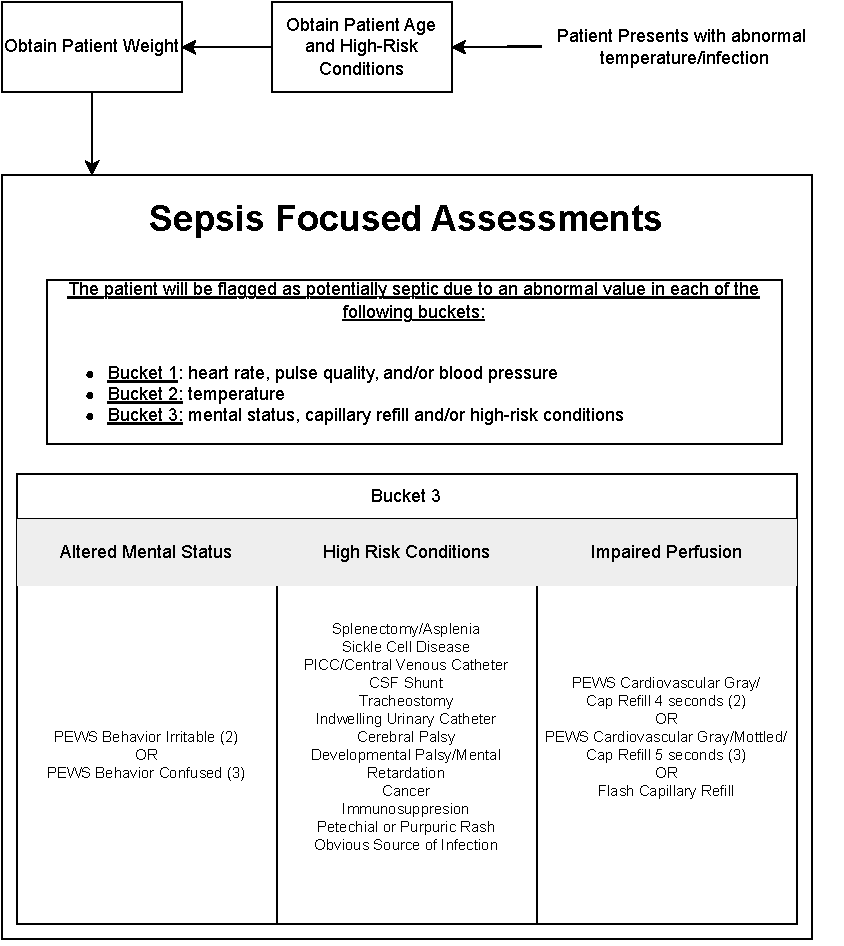
\includegraphics[width=\textwidth]{sepsis-screening-osf}
    \end{figure}
  \column{0.45\textwidth}
    \tiny
    \begin{tabular}{ | c || c | c | }
      \hline
      \textbf{Age}            & \textbf{Heart Rate}    & \textbf{Temp}  \\
      \hline
      $0d - 1m$               & $>205$                 & $<36 \text{ or } >38$ \\
      \hline
      $\geq 1m - 3m$          & $>205$                 & $<36 \text{ or } >38$ \\
      \hline
      $\geq 3m - 1y$          & $>190$                 & $<36 \text{ or } >38.5$ \\
      \hline
      $\dots$                 & $\dots$                & $\dots$ \\
      \hline
      $\geq 13y$              & $>100$                 & $<36 \text{ or } >38.5$ \\
      \hline
    \end{tabular}
  \end{columns}
\end{frame}

\begin{frame}{Guidelines-based Computerized Decision Support (CDSS)}
  Systems that codify BPGs to provide healthcare providers with situation-specific advice.
  \begin{itemize}
    \item BPG-adherence is difficult to achieve in practice.
    \item CDSSs integrate BPGs with existing care-flow and make them readily
      accessible.
    \item Reduce Preventable Medical Errors \cite{GargJAMA06,KawamotoBMJ05} and improve adherence to BPGs \cite{BenettJAMIA16,SahotaJIS11}.
  \end{itemize}
  \pause
  A typical CDSS consists of:
  \begin{itemize}
    \item A translation of the BPG into a computable medium (medical-logic).
    \item Integration with external data sources such as sensors and electronic
      records.
   \item A User-Interface for healthcare providers.
  \end{itemize}
\end{frame}

\begin{frame}{Computer Interpretable Guidelines}
  \begin{itemize}
    \item Typically, a conventional programming language
      is used for medical-logic, leading to an
      \alert{specification-implementation} gap.
    \pause
    \item Computer Interpretable Guidelines address this gap.
    \item Ensures that medical-logic has intended semantics.
  \end{itemize}
\end{frame}

\begin{frame}{Computer Interpretable Guidelines}
  \begin{itemize}
    \item Typically, a conventional programming language
      is used for medical-logic, leading to an
      \alert{specification-implementation} gap.
    \pause
    \item Computer Interpretable Guidelines address this gap.
    \item Ensures that medical-logic has intended semantics.
  \end{itemize}
\end{frame}

\begin{frame}[allowframebreaks]{References}
  \bibliography{references}
\end{frame}
\end{document}
